\chapter{Results}
The results stem from static configurations and dynamic parametrization for each training strategy.
The training set was decreased from 50000 to 12500, the test set from 10000 to 2500 data points.

Notably, the displayed values are one of many produced results and may vary from execution to execution. The programs can be found in the accompanying IPYNB/PY files, located in the ''src'' directory of the repository.
Results can be found in the ''log'' directories. The results referenced in the following context are taken from ''log-win\_advanced\_2''.\\

The Keras-driven neural network is the main focus of the experimentation. There are three main phases during the algorithm.

First, we create a standard, sequential model for generating results, which also serve as a 
reliable reference for other approaches. The basic model always uses the same parameters and layers.

Secondly, we run hyperparameter evaluation using the \href{https://keras.io/keras_tuner/}{keras\_tuner} library, to find more accurate models. The model resembles the standard model, with deviations in activation functions, dropout and learning rates, and units in the dense layer, as well as randomized deactivation of whole layer structures.
While almost every aspect of the model can be adjusted (see Overengineered Model), the more fundamental approach (Hyper model) allowed for better training times while being similarly efficient in its search.
The Hyper model is used for the three search strategies including Random Search, Bayesian Optimization, and \href{https://arxiv.org/abs/1603.06560}{Hyperband}

Thirdly, utilizing the findings by the hyperparameter search, a model is created and trained using the most optimal setup found during the evaluation.
The model with the highest accuracy score of the three mentioned strategies is chosen as the most optimal model.
For reference, the optimized model for the following results was automatically assigned by the algorithm, which is the Hyperband-Search Trial 47.
It uses the following configuration:
\begin{center}
  \begin{verbatim}
    Standard Model      |    Optimal Model
    --------------------+--------------------
    Conv2D(relu)        | Conv2D(relu)
    Conv2D(relu)        | Conv2D(relu)
    MaxPooling2D        | MaxPooling2D
    Dropout(0.25)       | Dropout(0.3)
    Flatten()           | Flatten()
    Dense(256,relu)     | Dense(128,sigmoid)
    Dense(256,relu)     | Dense(128,sigmoid)
    Dense(10,softmax)   | Dense(10,sigmoid)
    --------------------+--------------------
    learnrate:  0.0001  |  0.001   
  \end{verbatim}
\end{center}

\begin{table}[H]
  \centering
  \begin{tabular}{|l|l|l|l|l|}\hline
                        & \multicolumn{2}{|c|}{Standard Model}      & \multicolumn{2}{|c|}{Optimized Model} \\\hline
      Training time     & \multicolumn{2}{|l|}{493.6614336967468s}  & \multicolumn{2}{|l|}{290.2278664112091s}\\\hline\hline
      Model             & \multicolumn{1}{|c|}{Dataset}             & \multicolumn{1}{|c|}{Exec. Time}          & \multicolumn{1}{|c|}{Accuracy}            & \multicolumn{1}{|c|}{Loss} \\\hline
      Standard Model    & Train                                     & 7.391666650772095  & 0.7254980206489563  & 0.8031874299049377 \\
      Optimized Model   & Train                                     & 2.7842016220092773  & 0.9039123058319092  & 0.302592009305954 \\
      Standard Model    & Test                                      & 1.7537829875946045  & 0.6062424778938293  & 1.110999345779419 \\
      Optimized Model   & Test                                      & 0.6126744747161865  & 0.6202480792999268  & 1.2597756385803223 \\\hline
    \end{tabular}
  \caption{Training time, validation time, accuracy and loss for the standard and the optimized neural network model.}
  \label{tab:std_opt_model_comparison}
\end{table}

\begin{table}[H]
  \centering
  \begin{tabular}{|l|l|l|l|}\hline
    \multicolumn{1}{|c|}{Rank} & \multicolumn{1}{|c|}{HPS Strategy}   & \multicolumn{1}{|c|}{Accuracy} & \multicolumn{1}{|c|}{Loss} \\\hline
    1 & Random Search &  0.42296919226646423 &  1.9702255725860596 \\
    2 & Random Search &  0.35334134101867676 &  1.8446855545043945 \\
    3 & Random Search &  0.27050819993019104 &  7.551784038543701 \\\hline
    1 & Bayesian Optimization &  0.4233693480491638 &  2.0376853942871094 \\
    2 & Bayesian Optimization &  0.43017205595970154 &  2.0165903568267822 \\
    3 & Bayesian Optimization &  0.4337735176086426 &  2.024582624435425 \\\hline
    1 & Hyperband &   0.6166466474533081 &  1.1819623708724976 \\
    2 & Hyperband &  0.5922368764877319 &  1.2619372606277466\\
    3 & Hyperband &  0.5314125418663025 &  1.2906620502471924\\\hline
  \end{tabular}
  \caption{Small excerpt of the hyperparameter evaluation logs -- The three best models per strategy and their performances on accuracy and loss.}
  \label{tab:hps_strategy_comparison}
\end{table}

Surprisingly, the keras\_tuner algorithm considered the Bayesian Optimization with lower accuracy as the better model. 

The following visualizations further aid the understanding of the results and depict the difference in model fitting -- the optimized 
variant reaches a high point of validation accuracy very fast but does not improve afterward.
Given the difference in training and validation, this may indicate overfitting.
Interestingly, there is also a model (\ref{fig:confusion_matrix_overview_err} -- see log-win\_err\_2) which seemingly had high accuracy. Yet, the actual mapping was entirely incorrect.

\begin{figure}[H]
  \centering
  \begin{minipage}{.5\textwidth}
    \centering
    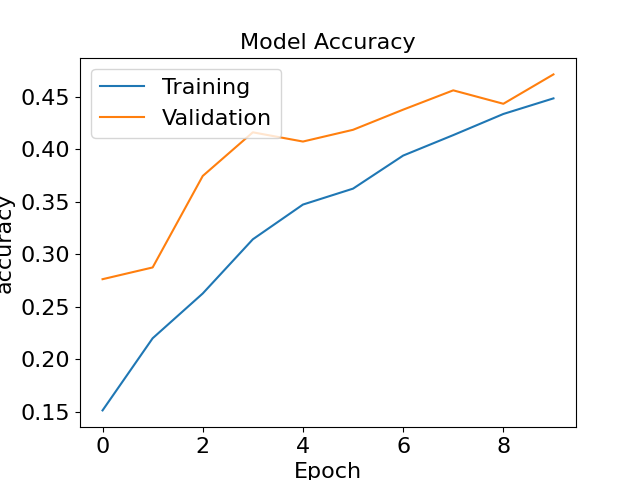
\includegraphics[width=1.0\linewidth]{img/training_history_standard.png}
    \label{fig:training_history_standard}
  \end{minipage}%
  \begin{minipage}{.5\textwidth}
    \centering
    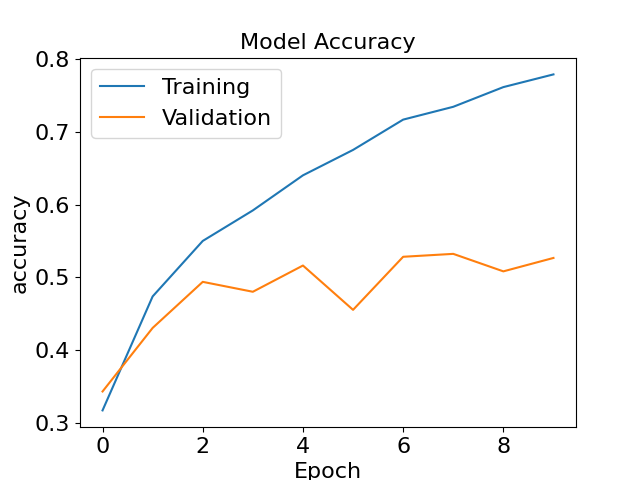
\includegraphics[width=1.0\linewidth]{img/training_history_optimal.png}
    \label{fig:training_history_optimal}
  \end{minipage}
  \caption{Training accuracy score comparison inbetween default network (left) and optimized network (right) parametrization.}
  \label{fig:training_history_overview}
\end{figure}

% Overfeed linewidth for better readability
\begin{figure}[H]
    \centering
    \begin{minipage}{.5\textwidth}
      \centering
      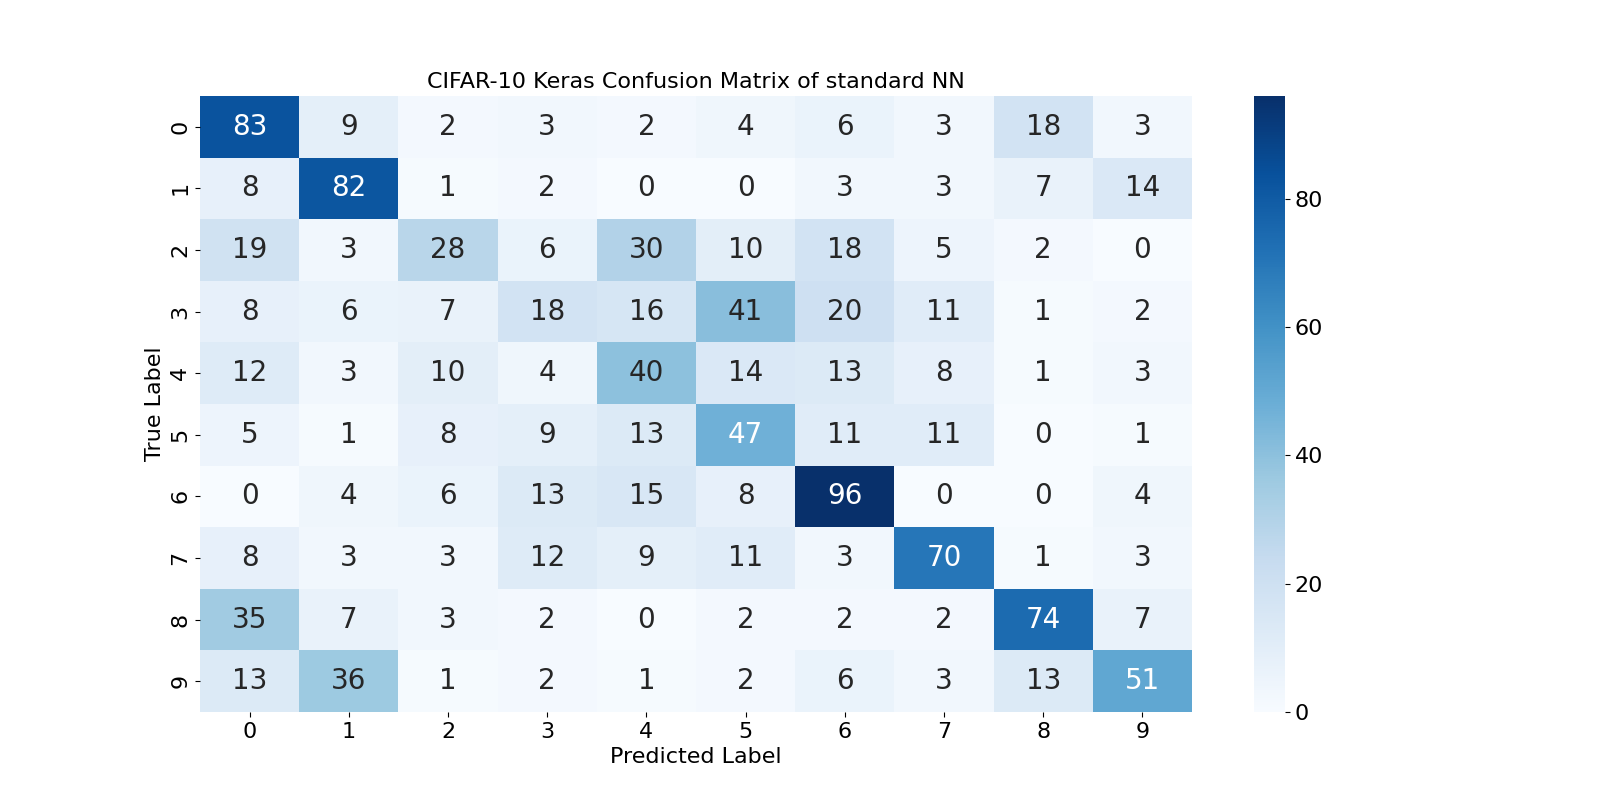
\includegraphics[width=1.25\linewidth]{img/ConfusionMatrix_standard.png}
      \label{fig:confusion_matrix_standard}
    \end{minipage}%
    \begin{minipage}{.5\textwidth}
      \centering
      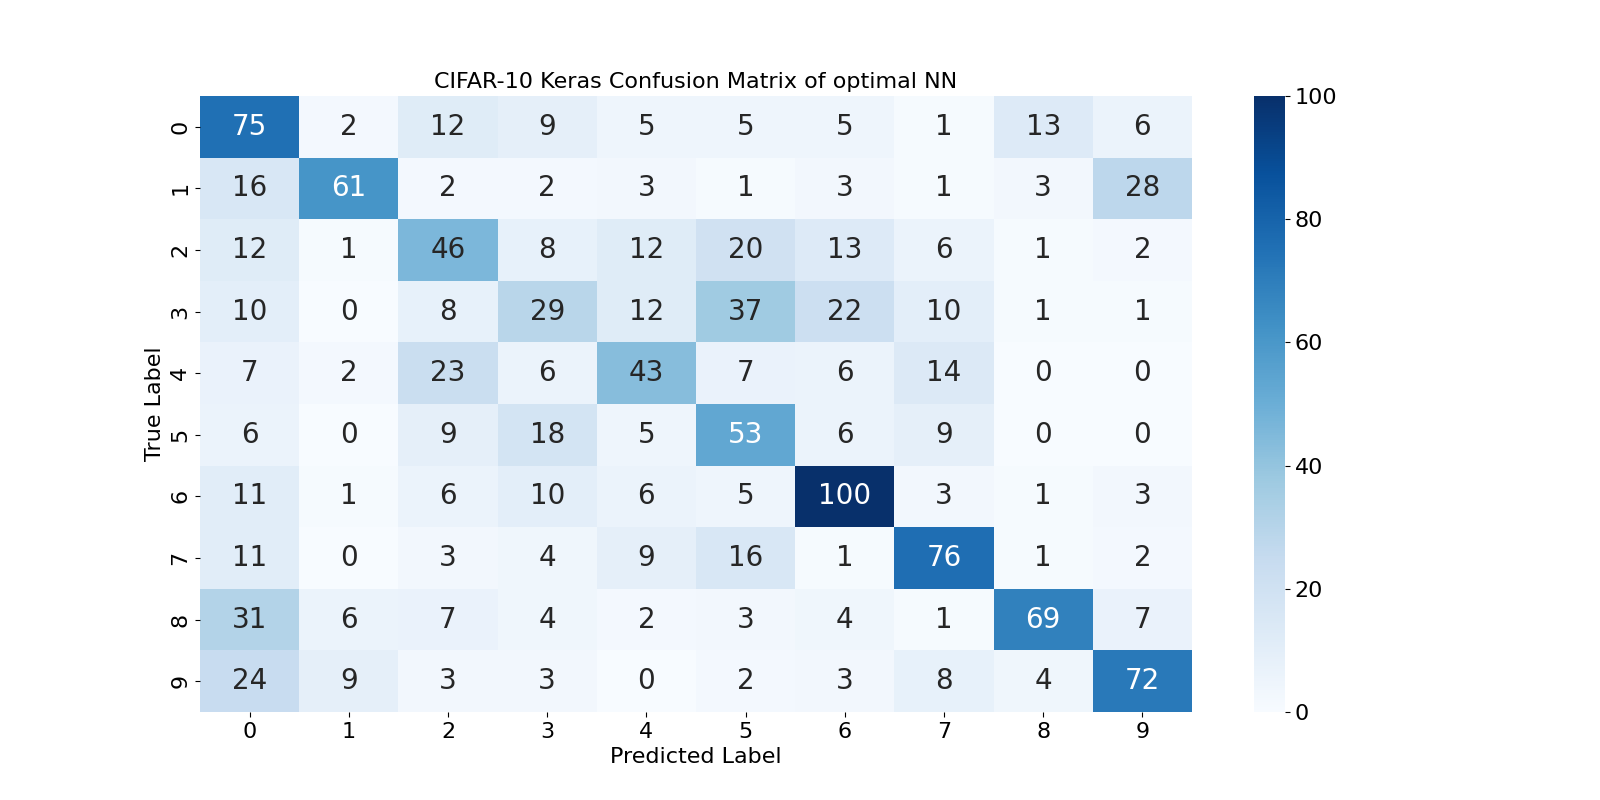
\includegraphics[width=1.25\linewidth]{img/ConfusionMatrix_optimal.png}
      \label{fig:confusion_matrix_optimal}
    \end{minipage}
    \caption{Confusion matrix comparison inbetween default network (left) and optimized network (right) parametrization.}
    \label{fig:confusion_matrix_overview}
\end{figure}


\begin{figure}[H]
  \centering
  \begin{minipage}{.5\textwidth}
    \centering
    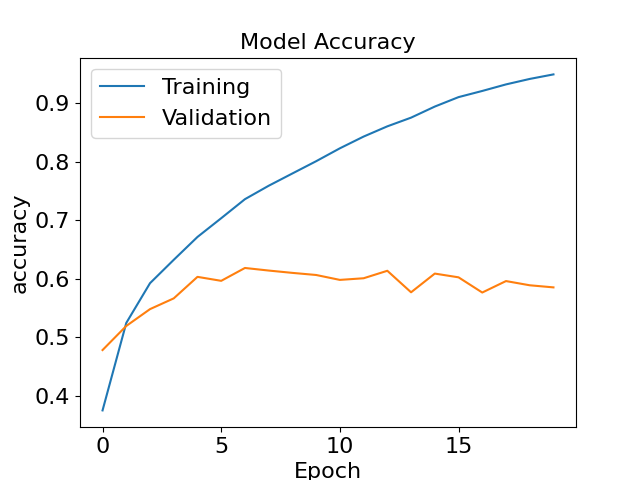
\includegraphics[width=1.0\linewidth]{img/training_history_optimal_err.png}
    \label{fig:training_history_optimal_err}
  \end{minipage}%
  \begin{minipage}{.5\textwidth}
    \centering
    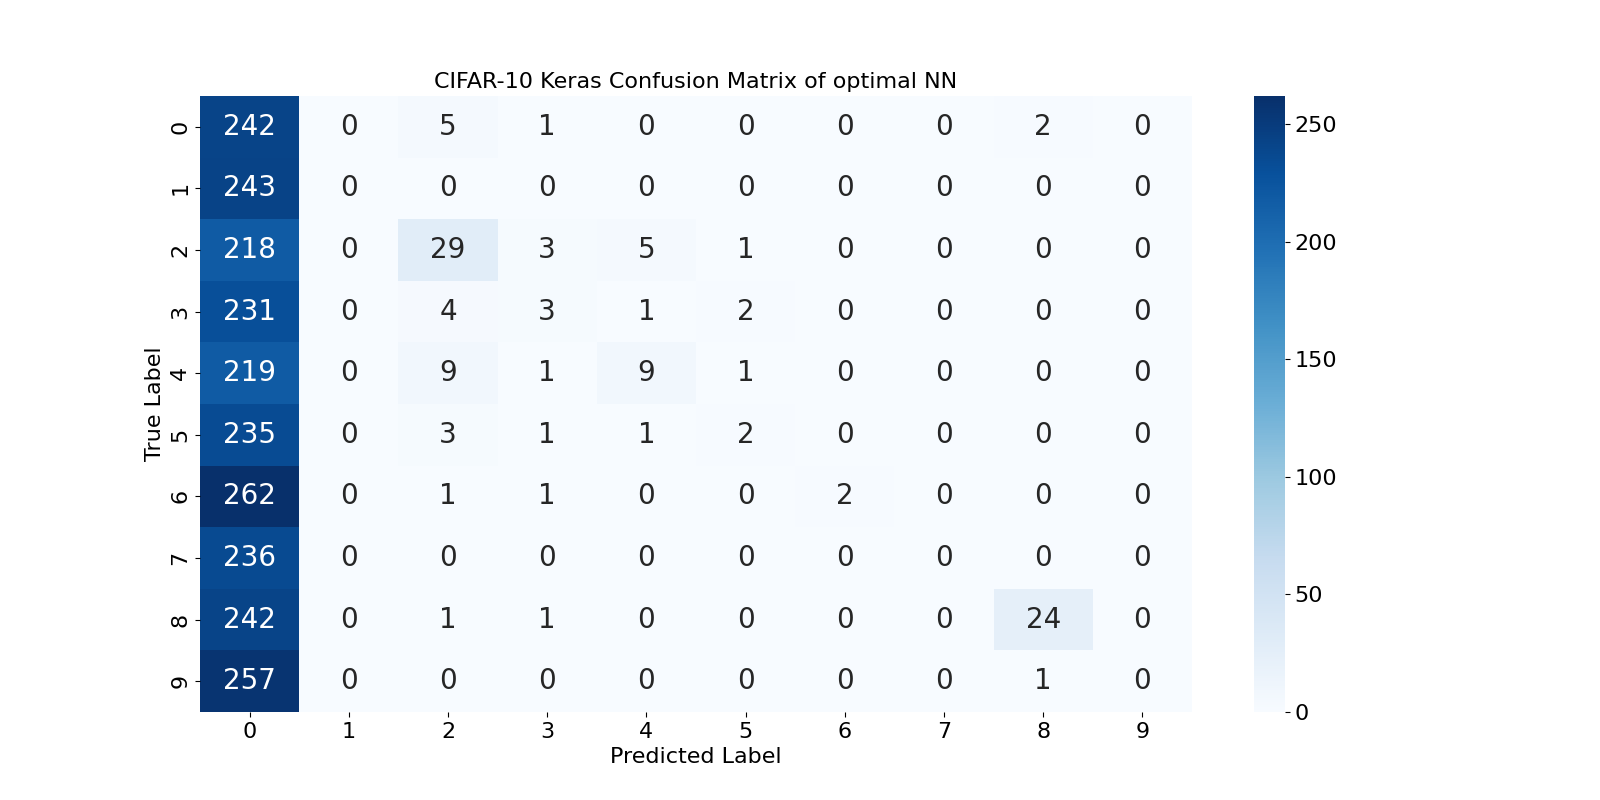
\includegraphics[width=1.25\linewidth]{img/ConfusionMatrix_optimal_err.png}
    \label{fig:confusion_matrix_optimal_err}
  \end{minipage}
  \caption{Training history (left) and coresponding confusion matrix (right) for a theoretically ''good'' model.}
  \label{fig:confusion_matrix_overview_err}
\end{figure}